\documentclass{article}

% Language setting
% Replace `english' with e.g. `spanish' to change the document language
\usepackage[english]{babel}

% Set page size and margins
% Replace `letterpaper' with `a4paper' for UK/EU standard size
\usepackage[a4paper,top=3cm,bottom=3.5cm,left=3cm,right=3cm,marginparwidth=2cm]{geometry}

% Useful packages
\usepackage{amsmath}
\usepackage{graphicx}
\usepackage[colorlinks=true, allcolors=blue]{hyperref}

\title{ASML:Classification Assessment}
\author{Xiaoning Nie. (cshb26)}

\begin{document}
\maketitle

\ 


\section{Executive Summary}

Imagine you are a hotel manager and you want to know if your guests will cancel their orders after booking. Call each customer to ask if they want to cancel their order? That's not practical. It can actually be solved quite well. A computer can help you with this repetitive task, and given enough food - the datasets - it will do the job brilliantly.

This project is all about using a dataset from a hotel to analyse the likelihood of future guests making a booking withdrawal. The dataset contains 119,390 pieces of data, each containing 32 features such as hotel type, guest payment method, number of guests, guest wait time for confirmation, etc. Some of these features are related to cancellations and some are not.	

What this project did was to filter out the relevant features and feed them to a computer, which generated a model that could be used to predict whether a guest would cancel in the future, and then optimise it to improve the accuracy of the computer's predictions. At the end of the project, the model achieved the desired accuracy rate!!!!-----???, so it can be considered a successful model.

The use of computers to analyse data can be very challenging but also very interesting as when analysing a dataset, we can visualise the data to make our analysis more sufficient and efficient. For example, when first reading in the dataset, we can draw a few features of interest to see the weight of each attribute, as shown in Figure 1 for total\_nights and adr, the average daily rate. It is clear from the plot that the vast majority of people choose to stay for less than 10 days and almost all hotels have an adr of no more than 300 per night.

\begin{figure}[h]
\centering
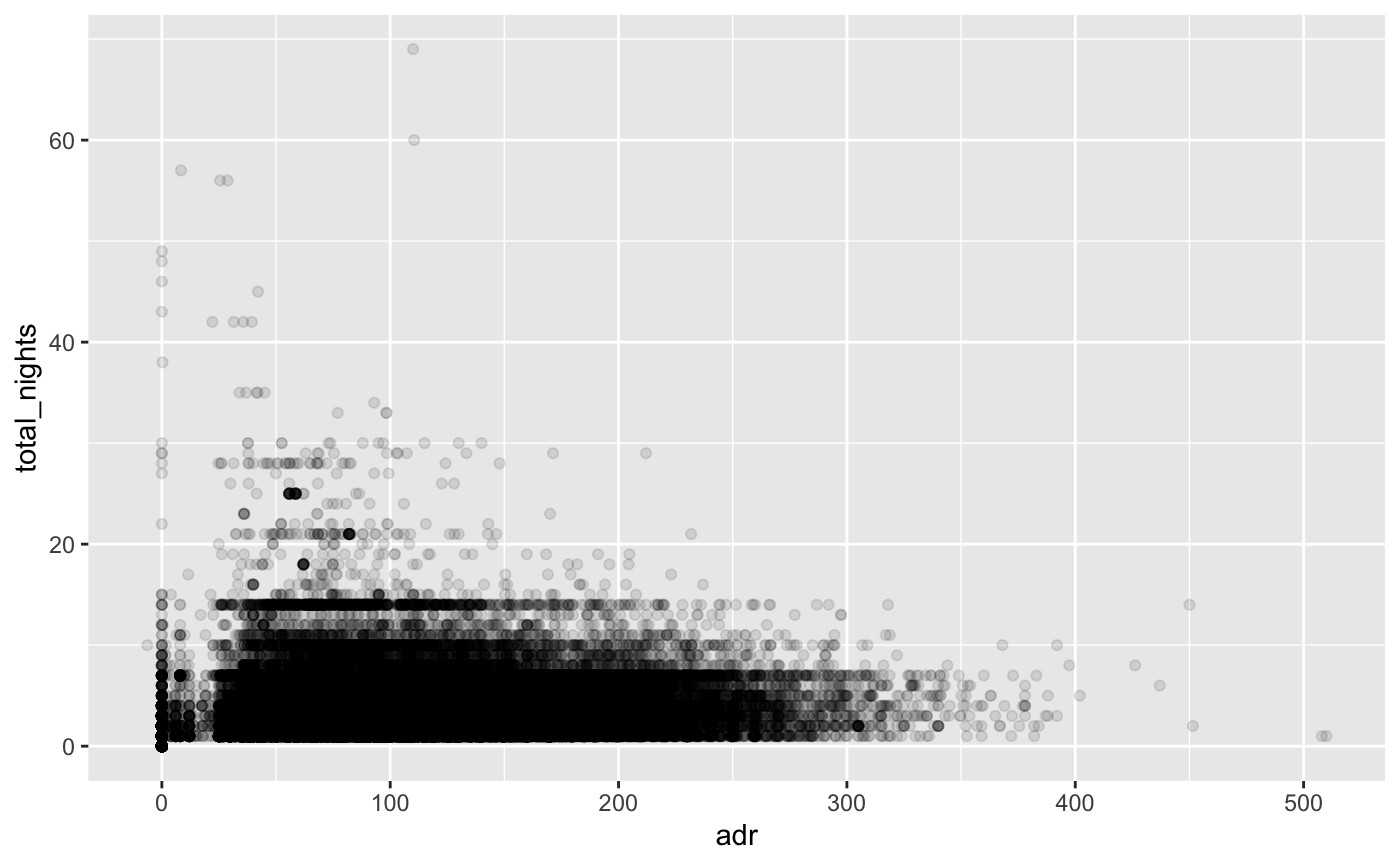
\includegraphics[width=12cm]{nightadr.png} %[图片大小]{图片路径}
\caption{Plot of total\_nights vs adr} %图片标题
\end{figure}


\ 

\section{Problem Description}

The dataset is a hotel dataset containing 119,390 data and 32 features detailing each guest's booking and itinerary information, which is used to train the model. In detail, 13 of these 32 features are of type character, 18 of type numeric and 1 of type Date, with one of the features of type numeric, is\_canceled, being intended to be predicted by modeling. Also, this dataset is of high quality with few missing values, which facilitates modeling. Figures 2, 3 and 4, 5 show the relationship between the data and predicted values for the numeric and character types respectively, and it is clear that certain features are not relevant to the predicted values and will be cleaned up later.

\begin{figure}[htbp]
\centering

\subfigure[]{
\begin{minipage}[h]{0.4\linewidth}
\centering
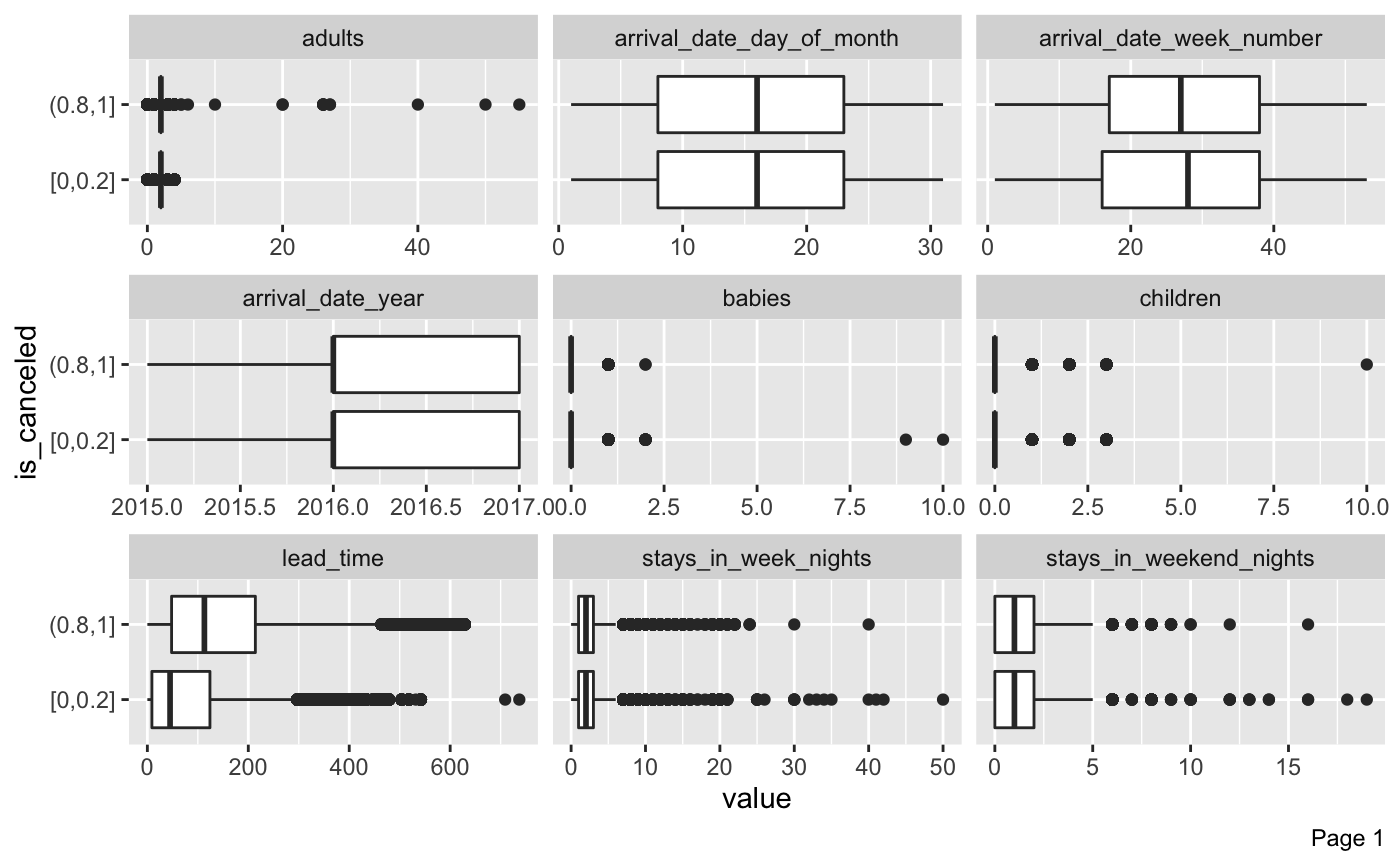
\includegraphics[width=2.5in]{datanum1.png}
\caption{P1 of numeric data}
\end{minipage}%
}%
\subfigure[]{
\begin{minipage}[h]{0.5\linewidth}
\centering
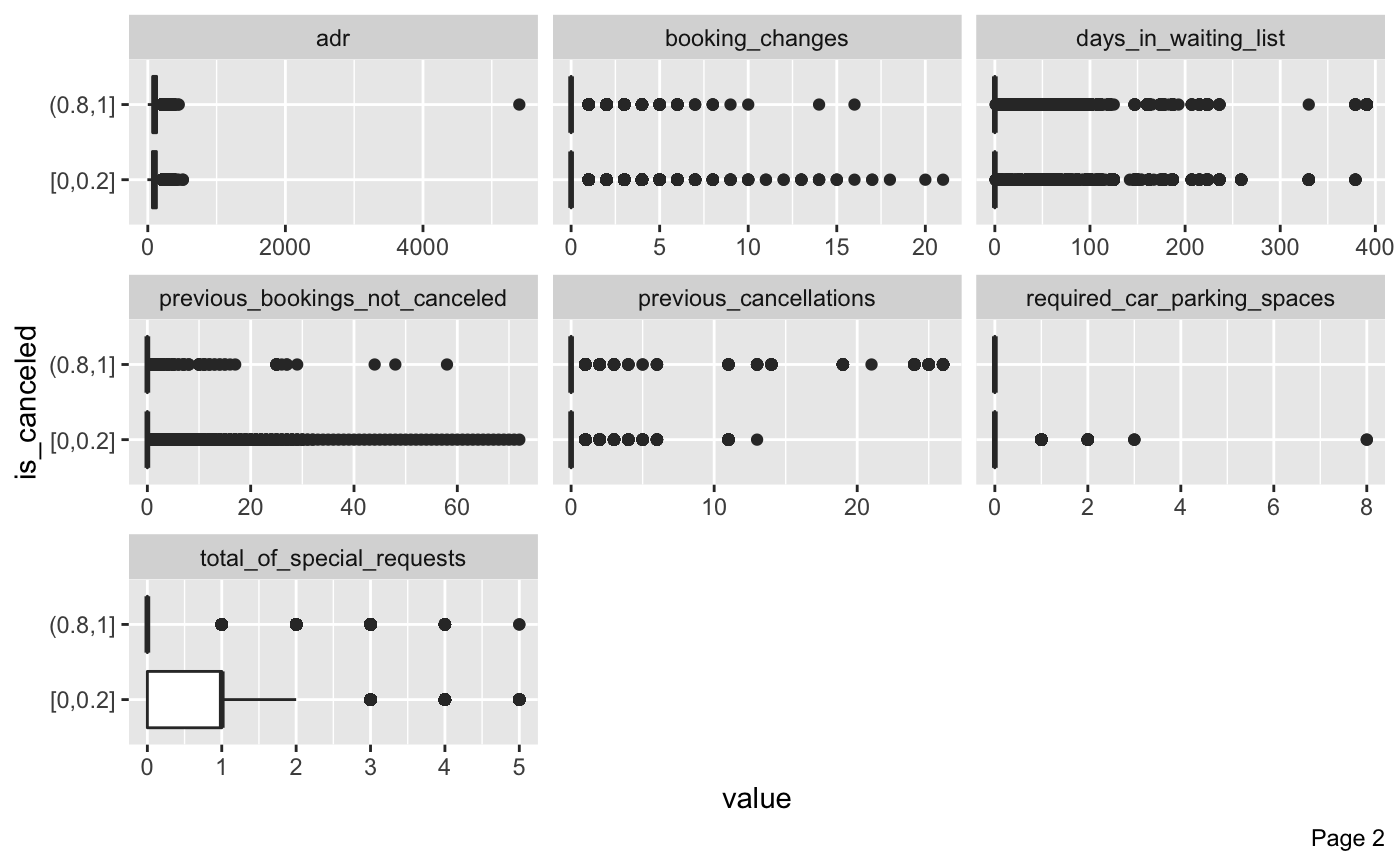
\includegraphics[width=2.5in]{datanum2.png}
\caption{P2 of numeric data}
\end{minipage}%
}%
\quad     %这个回车键很重要 \quad也可以
\subfigure[]{
\begin{minipage}[h]{0.5\linewidth}
\centering
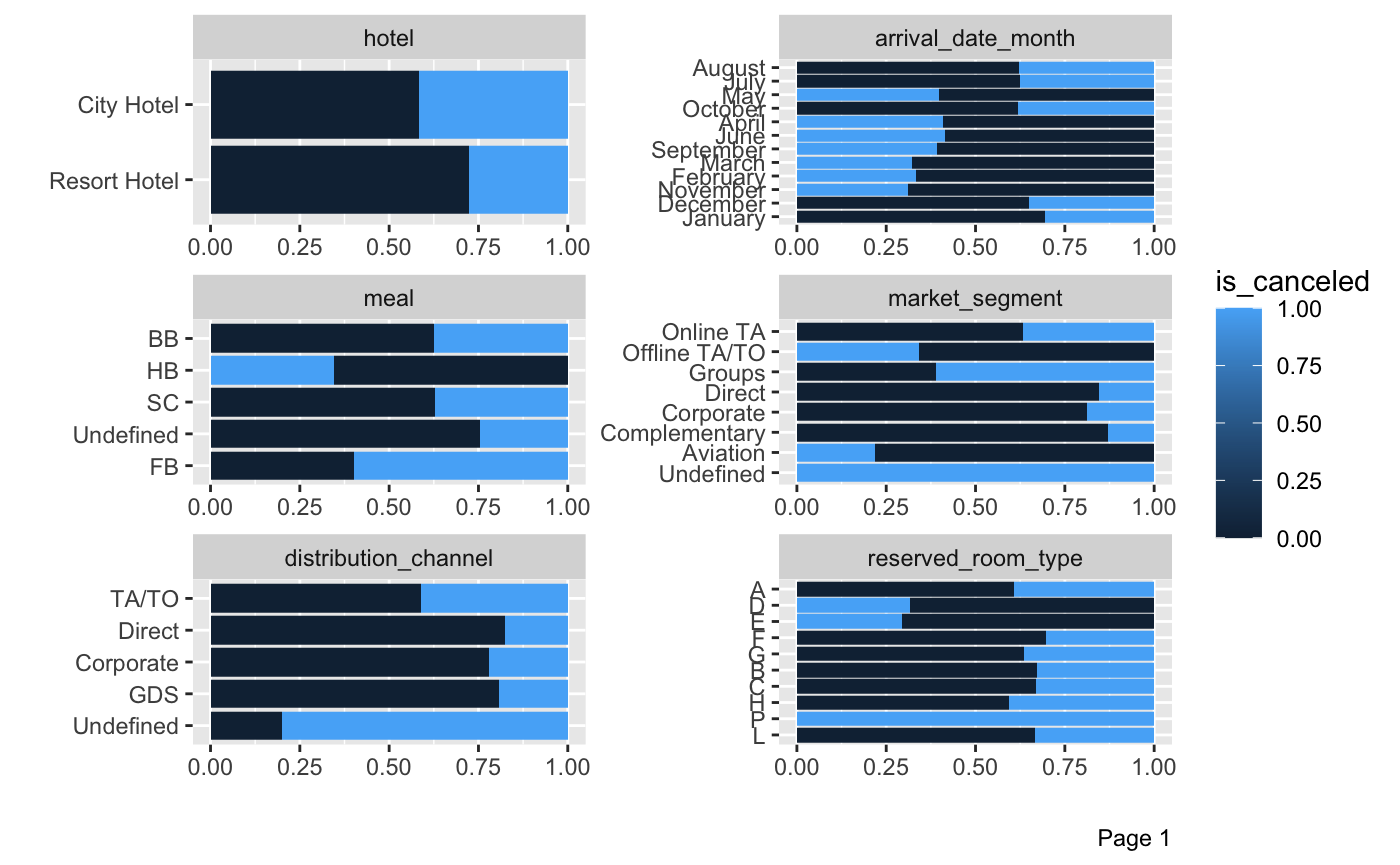
\includegraphics[width=3in]{datachar1.png}
\caption{P1 of categorical data}
\end{minipage}
}
\subfigure[]{
\begin{minipage}[h]{0.4\linewidth}
\centering
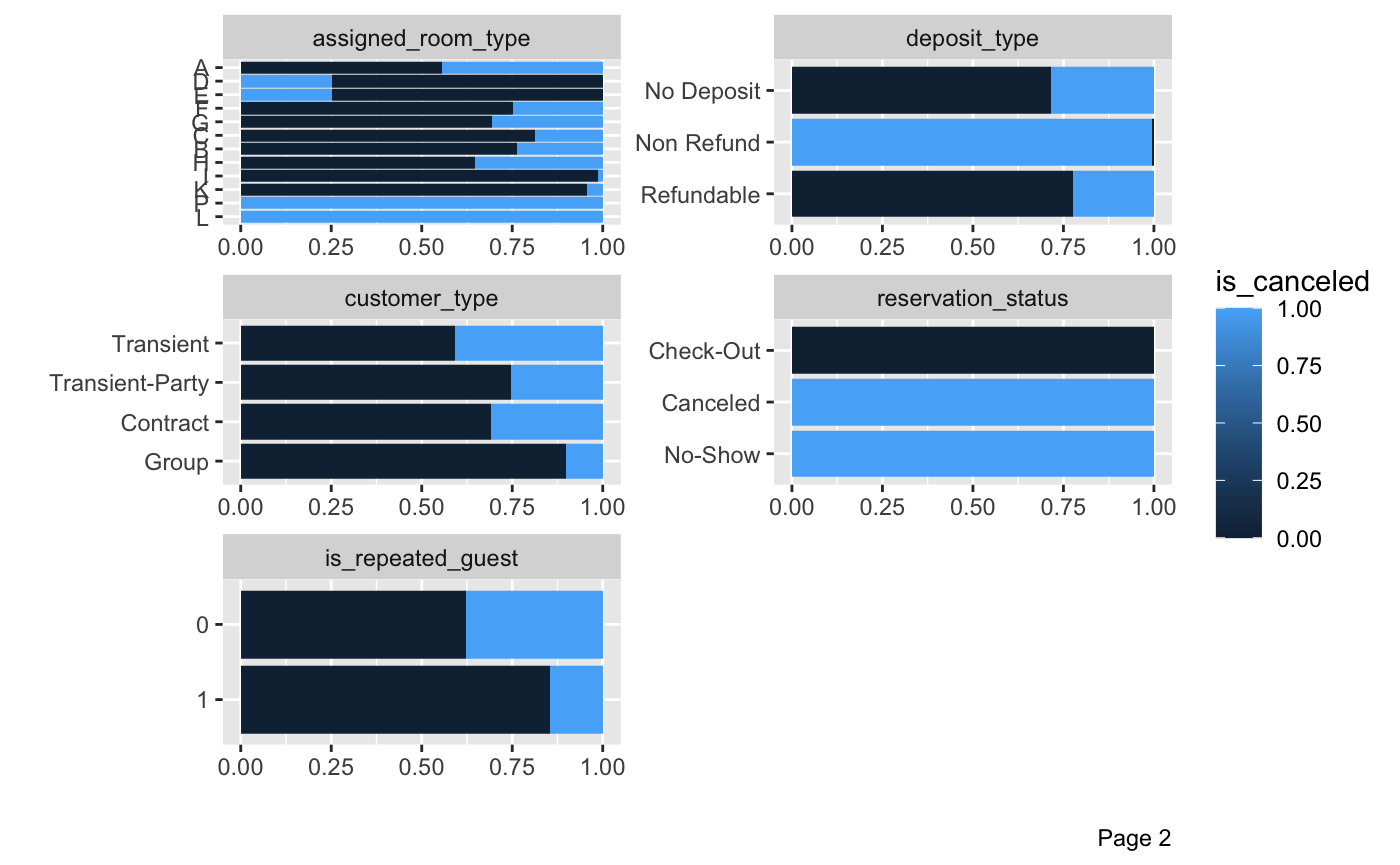
\includegraphics[width=3in]{datachar2.png}
\caption{P2 of categorical data}
\end{minipage}
}%

\centering
\end{figure}



\section{Model Fitting}

\subsection{Feature engineering}

\subsubsection{Data cleaning}

A look at the dataset reveals the following redundant features or non-relevant variables, so they are cleaned.

1. \verb|reservation_status| and \verb|reservation_status_date| are not meaningful to the predicted outcome and are therefore removed.

2. \verb|stays_in_weekend_nights| and \verb|stays_in_week_nights| have redundant information for the forecast, so \verb|total_nights| is set to replace them.

3. \verb|kids| is set to replace \verb|children| and \verb|babies|.

4. Set \verb|room_type| to 1 if \verb|reserved_room_type| and \verb|assigned_room_type| are the same, 0 if they are not.

5. Create a new variable \verb|parking| which is either \verb|parking| or \verb|none| depending on the value of \verb|required_car_parking_spaces|.

6. Convert \verb|arrival_date_month| to numeric type data.

7. \verb|country|, \verb|agent|, \verb|company|, \verb|date| and \verb|week| categories are too many to be considered and are therefore removed.


\subsubsection{Correlation analysis of the remaining variables}

The results shown in Figure 6 and 7 can be obtained by correlation analysis of the remaining variables, and it was judged that ** had a low correlation with the predicted results, so they were removed.

\begin{figure}[h]
\centering
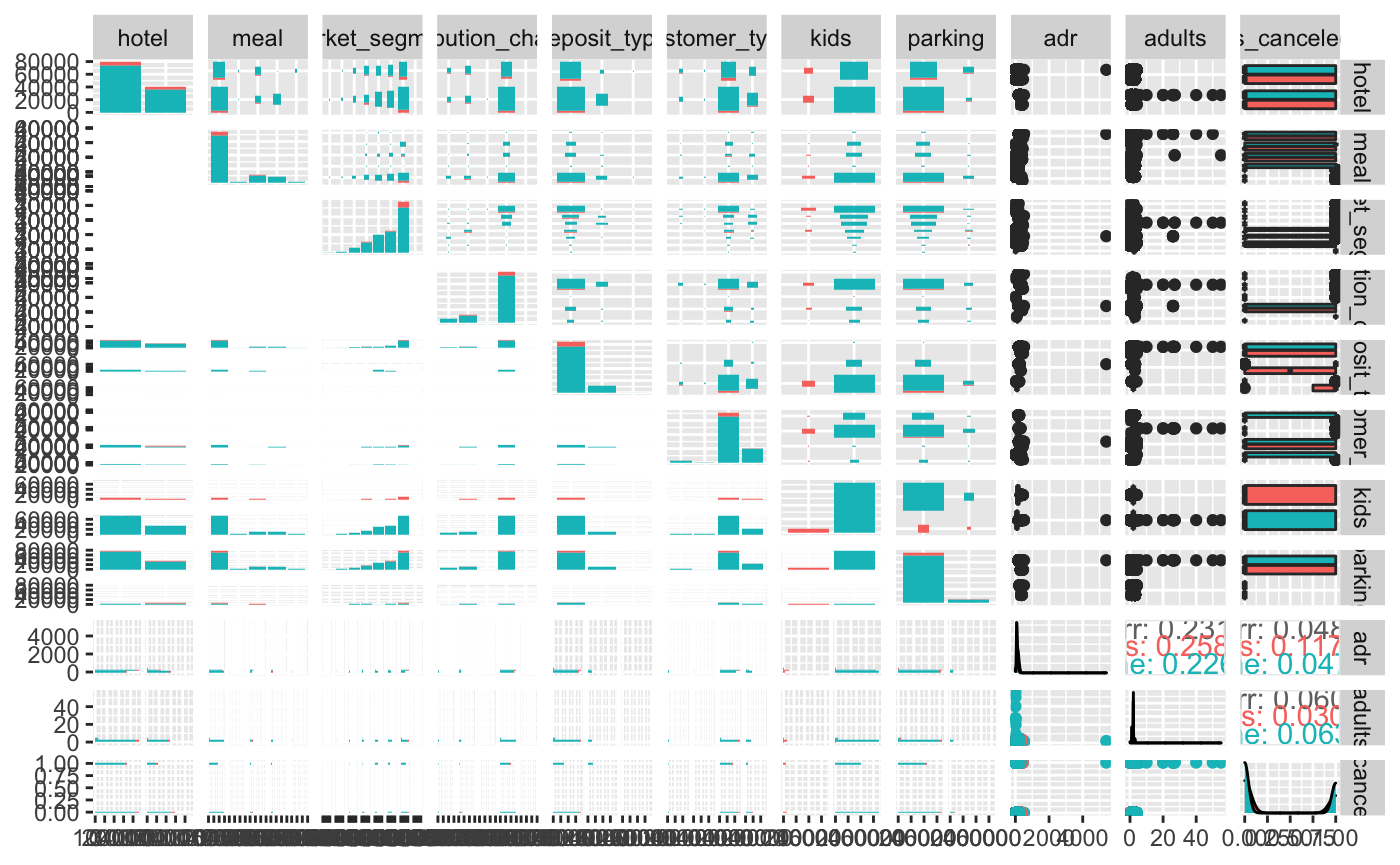
\includegraphics[width=10cm]{remain1.png} %[图片大小]{图片路径}
\caption{P1 of the analysis} %图片标题
\end{figure}

\begin{figure}[h]
\centering
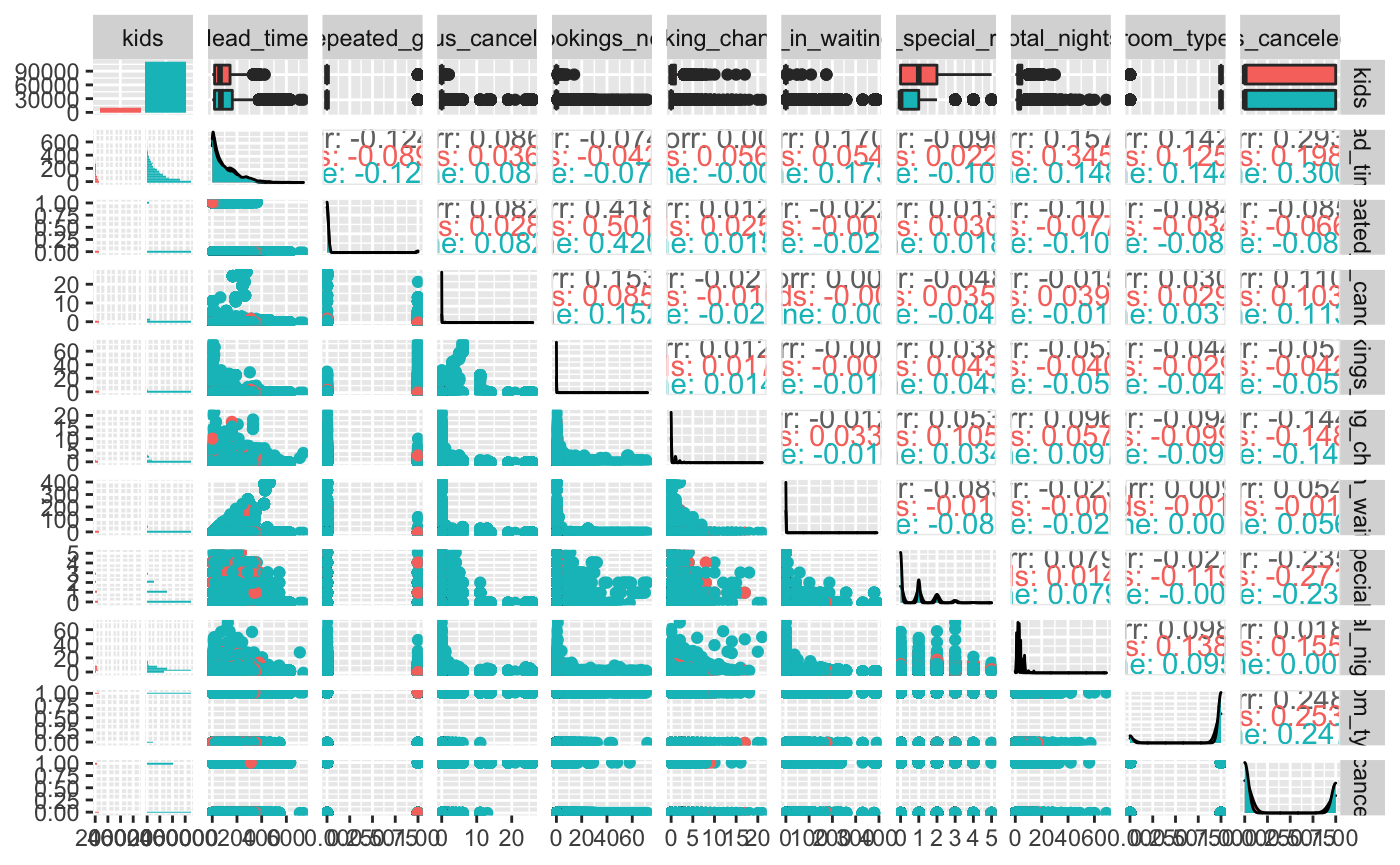
\includegraphics[width=10cm]{remain2.png} %[图片大小]{图片路径}
\caption{P2 of the analysis} %图片标题
\end{figure}

The above images show that there are several features such as \verb|hotel|, \verb|meal| and \verb|adr| that have low correlation with the predicted value, so they are removed here.


\subsubsection{Outlier handling}

The analysis yielded the following 2 outliers.

1. As shown in Figure 8, 99\% of \verb|days_in_waiting_list| are 0, which is not representative, so is deleted.

\begin{figure}[h]
\centering
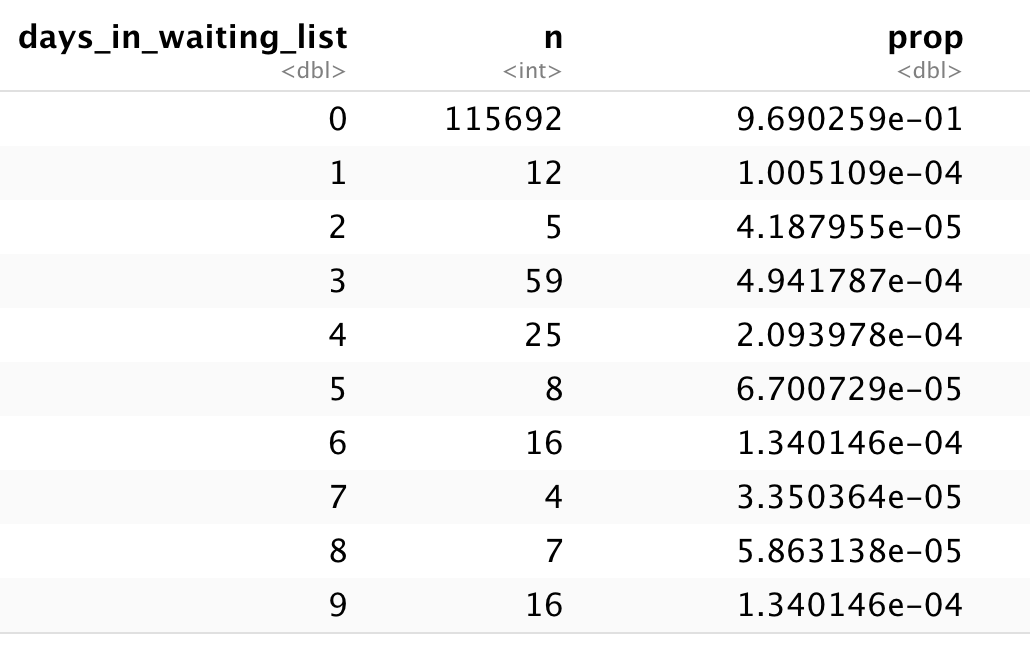
\includegraphics[width=6cm]{days.png} %[图片大小]{图片路径}
\caption{Percentage of each value in days\_in\_waiting\_list} %图片标题
\end{figure}

2. As shown in Figure 9, there are many values in the \verb|lead_time| category, so it was discretised and binned, i.e., the values of \verb|lead_time| were divided into 4 parts with equal frequency, and the values were replaced by categories 1-4 in order.

\begin{figure}[h]
\centering
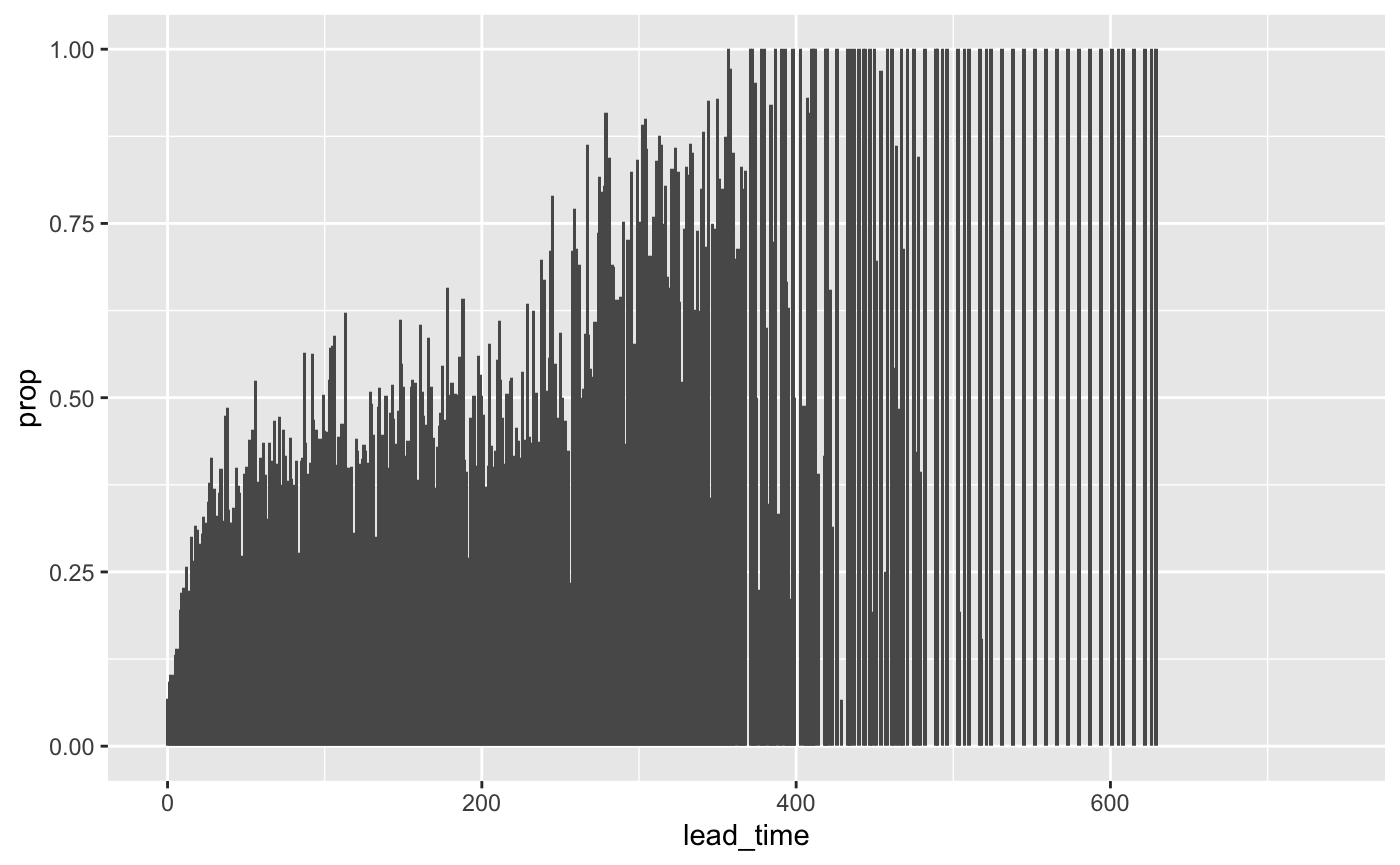
\includegraphics[width=8cm]{lead.png} %[图片大小]{图片路径}
\caption{Data of category lead\_time} %图片标题
\end{figure}



\subsection{Modeling}

Logistic regression was used to solve this problem based on the choice of the number of target predicted values, and the results are shown in Figure 10.

\begin{figure}[h]
\centering
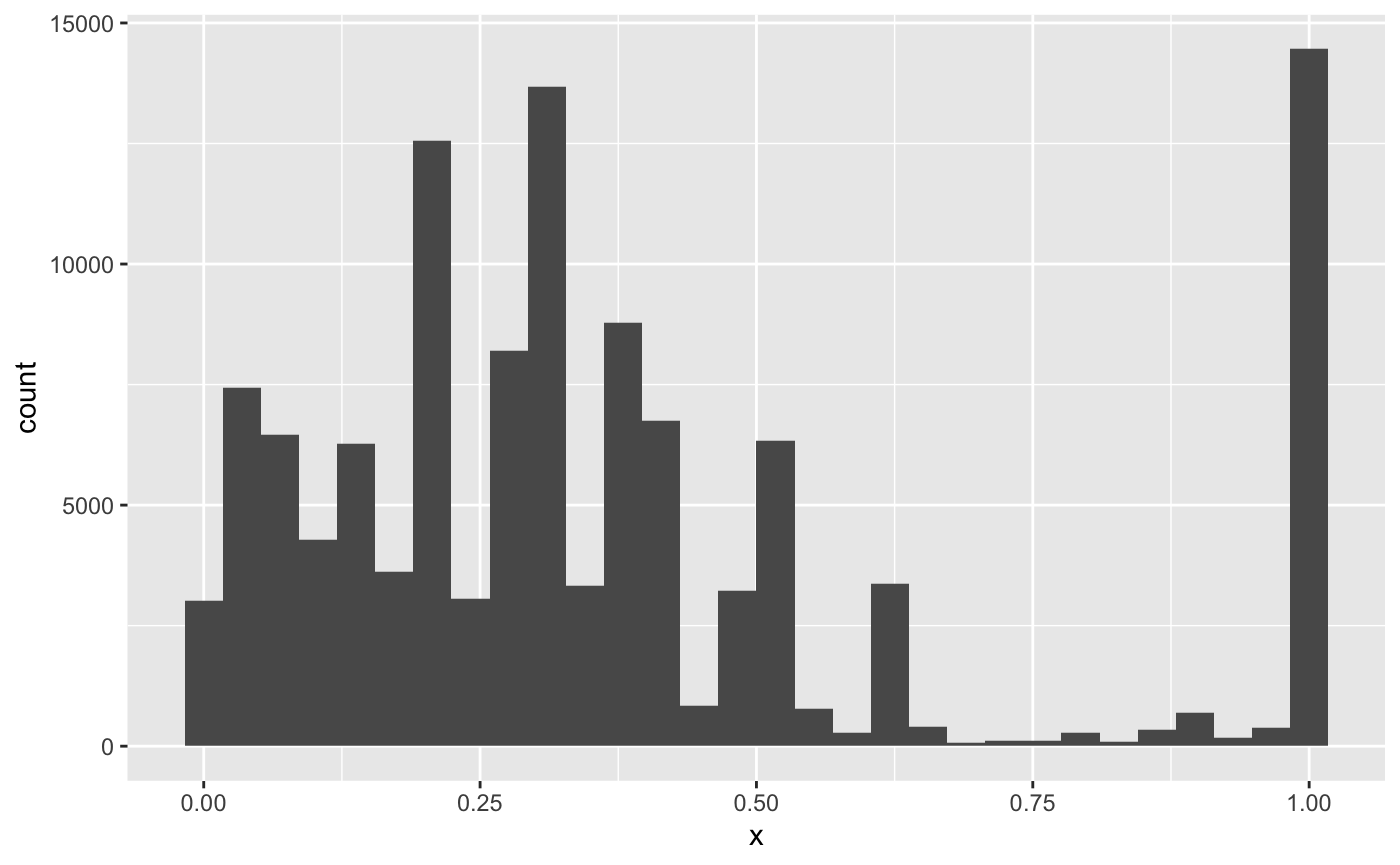
\includegraphics[width=8cm]{lrresult.png} %[图片大小]{图片路径}
\caption{Simple logistic regression result} %图片标题
\end{figure}

It can be seen that the model gives the probability of the full data and by setting the threshold to 0.5 the model prediction can be obtained.

The TPR of the model can be calculated as 93.58 and the FNR as 52.06, with an overall correct rate of 82\%, which seems good but could be improved.


\section{Model Improvements}

After the results of the simple logistic regression were obtained, a new solution using the cross-validation was devised to improve the accuracy, and this was the final model chosen. 

The specific algorithm is to classify using the classifier in the \verb|mlr3| package and obtain the final error rate by cross-validation.


\section{Performance Report}

\subsection{Model selection}
对于简单逻辑回归的模型来说,能够得到82\%的正确率已经是不错的成绩,但如果使用交叉验证后,成绩又会再次提高。

对于一般的数据集较小的问题来说,使用简单逻辑回归会使效率提高,因为速度较快,并且能够得到相对不错的成绩;但对于较大的数据集来说,使用如交叉验证的其他方法能够提高正确率。


\subsection{Model selection}
any post-model analysis such as tuning true/false positive rates (e.g would you be more worried about false negatives or false positives in this problem, and how could you address that concern).






\ 

\section{Reproducible code}


%\begin{figure}[h]
%\centering
%\includegraphics[width=12cm]{q1.png} %[图片大小]{图片路径}
%\caption{Plot of Question 1} %图片标题
%\end{figure}



\end{document}